\section{Umsetzung:}
\subsection*{Frontend:}
\begin{figure}[h!]
    \begin{minipage}[c]{0.5\textwidth}
      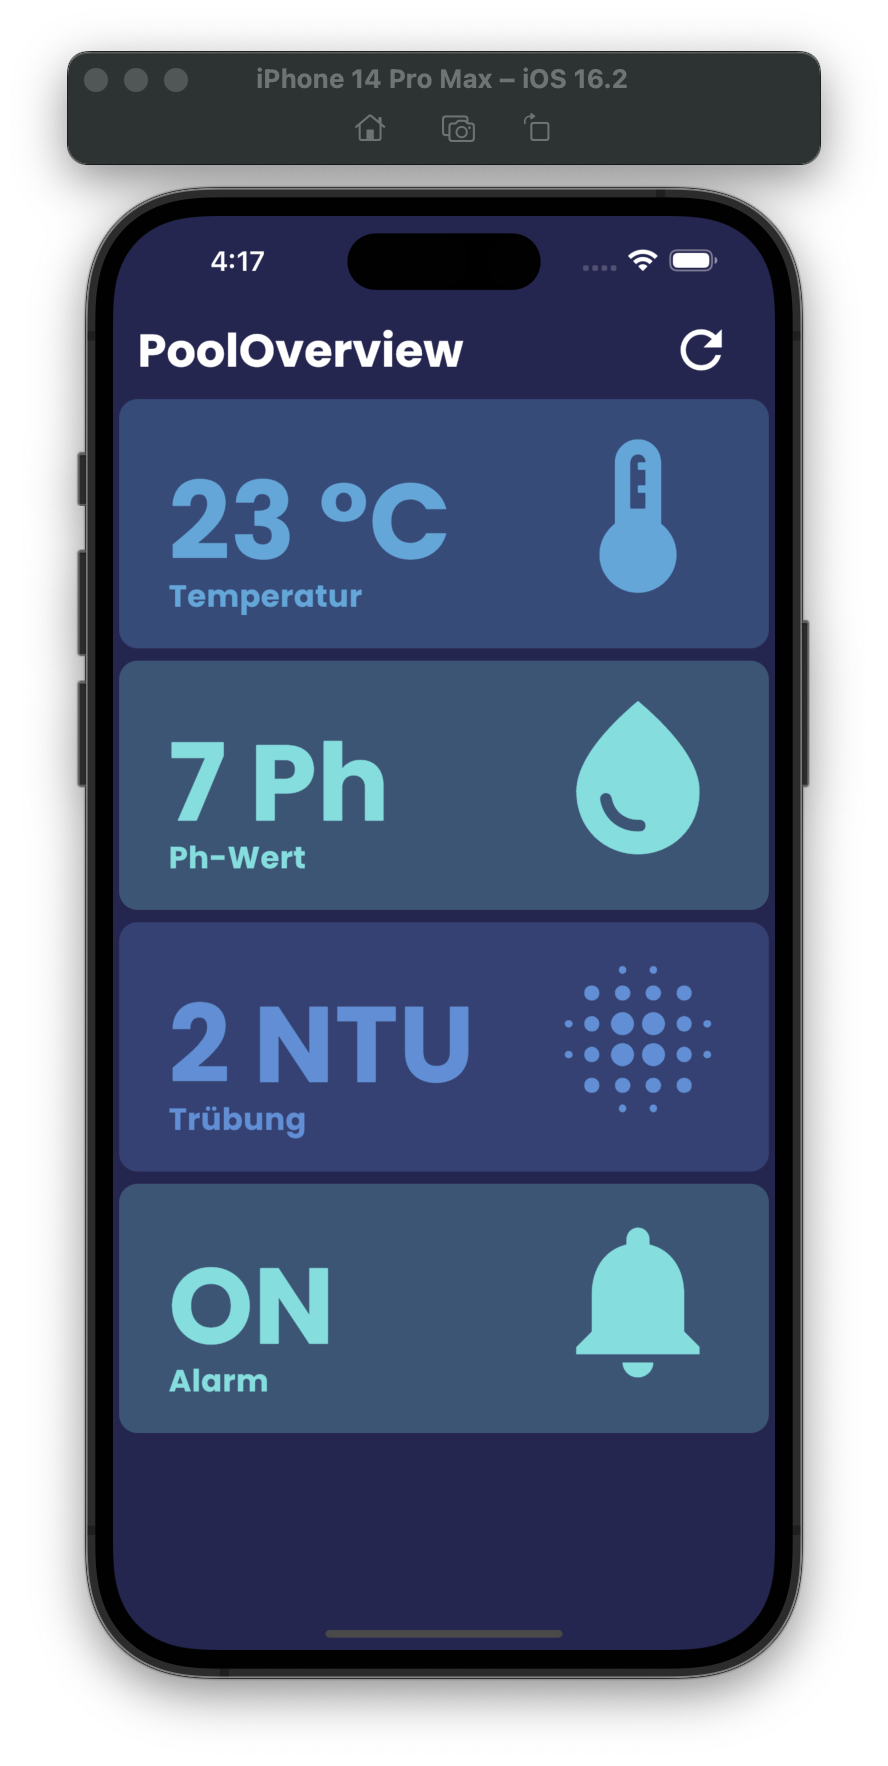
\includegraphics[width=\textwidth]{./pics/StartpageBild.png}
    \end{minipage}
    \begin{minipage}[c]{0.5\textwidth}
      \label{fig:Startpagebild}
      Der Home-Screen basiert auf einem Scroll-View,
      welches den Vorteil bietet ein einheitliches Design auf jeder Art von Bildschrimgröße zu gewährleisten, ohne die Lesbarkeit zu beeinträchtigen. 
      Ein ScrollView in Flutter ist ein Widget, das verwendet wird, um eine Liste von Elementen anzuzeigen, die größer sind als der verfügbare Bildschirm. 
      Es ermöglicht dem Benutzer, durch die Liste zu scrollen, um alle Elemente anzuzeigen. Es gibt verschiedene Arten von ScrollView in Flutter, darunter ScrollView, ListView, GridView und CustomScrollView. Das ScrollView enthält generisch selbst erstellte Objekte names DataCard.
    \end{minipage}
  \end{figure}
  \newpage
  \subsection*{DataCards:}
  \begin{figure}[h!]
    \begin{minipage}[c]{0.5\textwidth}
      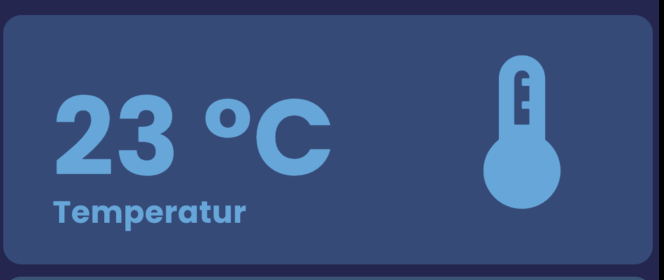
\includegraphics[width=\textwidth]{./pics/Bildschirm­foto 2023-03-24 um 16.25.49.png}
    \end{minipage}
    \begin{minipage}[c]{0.5\textwidth}
      \label{fig:DataCard}
      Das DataCard Widget in Flutter ist ein vorgefertigtes Material Design-Widget, das zur Darstellung von Informationen in einem Kartenformat verwendet wird. 
      Es besteht aus einer rechteckigen Box mit abgerundeten Ecken, die in der Regel eine Hintergrundfarbe, einen Titel, eine Beschreibung und optional eine Aktion oder einen Button enthält.
      Das DataCard Widget enthält verschiedene Eigenschaften, die angepasst werden können, um das Erscheinungsbild und das Verhalten der Karte zu steuern. Dazu gehören Eigenschaften wie Hintergrundfarbe, Ränder, Schatten, Größe, Padding und Ausrichtung.  
    \end{minipage}
  \end{figure}
DataCards verfügen über die Funktion „onPressed“ in der man angeben kann was geschieht, wenn man eine der 5 DataCards drückt. Wenn man eine DataCard die den Namen „Temperatur“, „Ph-Wert“ oder „Trübung“ drückt wird man an eine weitere Page der App weiter geleitet in der man Statistiken zu dem jeweiligen Wert erhält. Wenn man die DataCard mit dem Namen „Alarm“ drückt wird der Alarm den man erhält wenn verdächtige Bewegungen des Gyroskopssensors wahrgenommen werden aktiviert oder deaktiviert.
Die DataCards auf dem HomeScreen enthalten ansonsten den zuletzt gemessenen Wert, der durch einen WebSocket vom Backend bereitgestellt wird und stellen diesen dar. Die DataCards sind generisch erstellbar mit Übergabewerten, was eine einfache Vergrößerung des Funktionsumfangs des HomeScreens ermöglicht.
Die Icons die auf den DataCards zu sehen sind, werden von Google-Material-Icons bereitgestellt und werden mittels API in die App Ressourceneffizient implementiert.
\begin{figure}[h!]
    \begin{minipage}[c]{0.5\textwidth}
      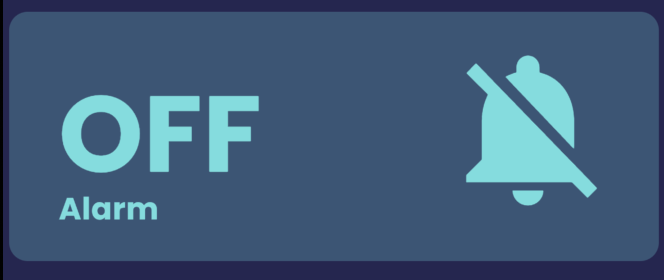
\includegraphics[width=\textwidth]{./pics/Bildschirm­foto 2023-03-24 um 16.22.40.png}
    \end{minipage}
    \begin{minipage}[c]{0.5\textwidth}
      \label{fig:AlarmOFF}
      So sieht die DataCard aus wenn man den Alarm durch drücken des Feldes deaktivert.
    \end{minipage}
\end{figure}
\newpage
\subsection*{Grafische Darstellung der Werte über Zeit:}

\begin{figure}[h!]
    \begin{minipage}[c]{0.4\textwidth}
      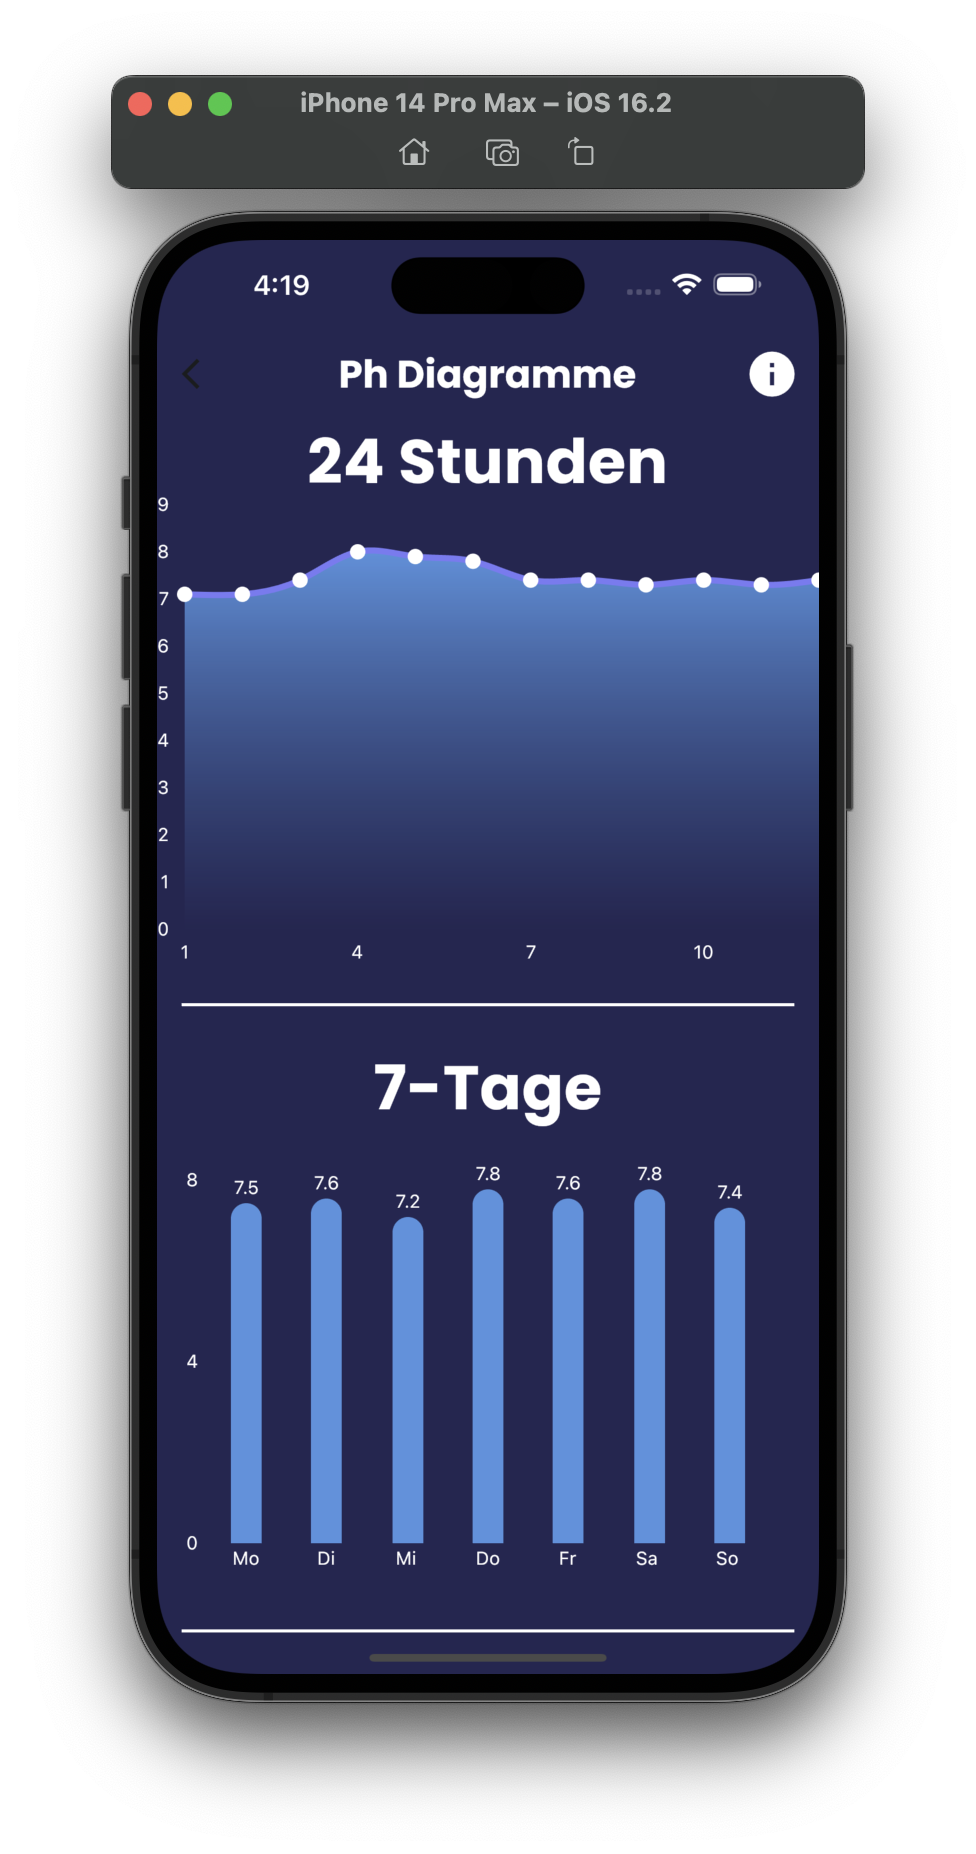
\includegraphics[width=\textwidth]{./pics/Diagramme1Bild.png}
    \end{minipage}
    \begin{minipage}[c]{0.5\textwidth}
      \label{fig:DigrammeApp1}
      Hier sind die Diagramme dargestellt auf die man durch das klicken der DataCards weiter geleitet wird. 
      Sie werden durch die Libraries "charts\_flutter" und "syncfusion\_flutter\_charts" bereitgestellt und mittels
      HTTP-Request befüllt und bei aufruf aktualisiert.

    \end{minipage}
\end{figure}
\begin{figure}[h!]
    \begin{minipage}[c]{0.4\textwidth}
      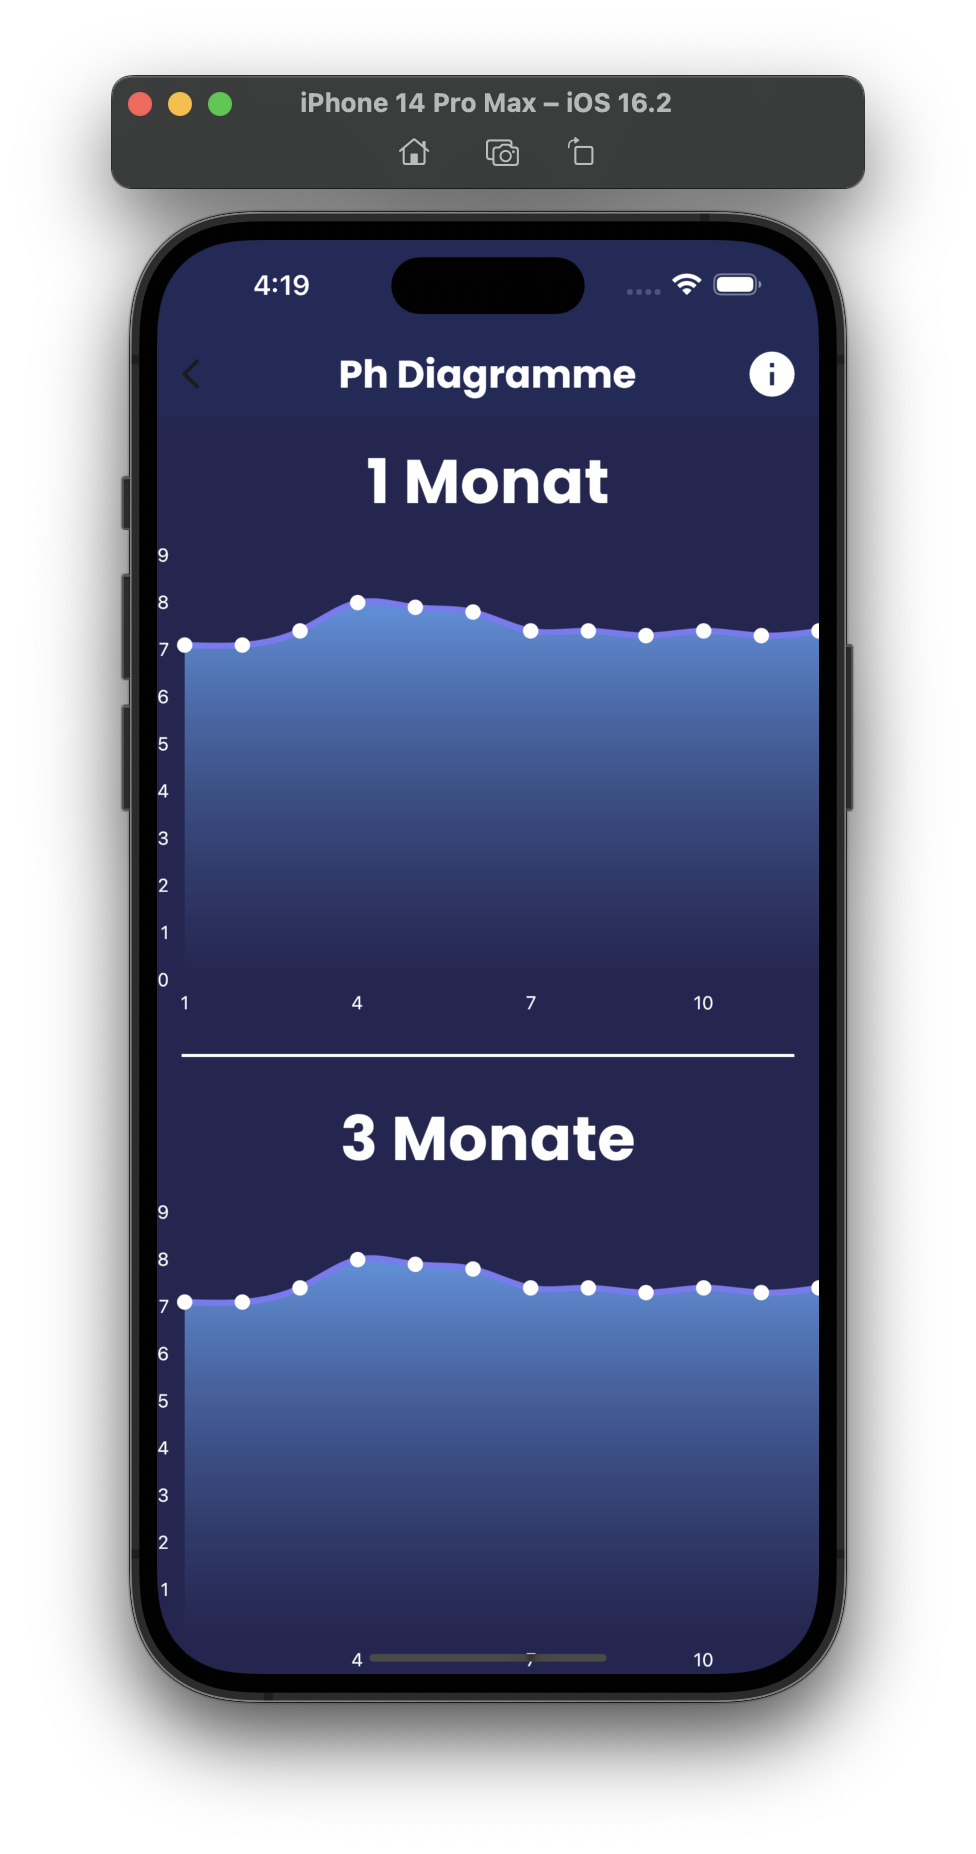
\includegraphics[width=\textwidth]{./pics/Diagramme2Bild.png}
    \end{minipage}
    \begin{minipage}[c]{0.5\textwidth}
      \label{fig:DiagrammeApp2}
      Nach dem Freunde Verwandte und Bekannte mittels mündlicher Umfrage befragt wurden, ist beschlossen worden, dass
      Diagramme in den Zeiträumen "24 Stunden", "7 Tage", "1 Monat" und "3Monate" angezeigt werden sollen.
      Diese Zeiträume waren am beliebtesten und sind wenn man die durchschnittliche Dauer einer Badesaison betrachtet am relevantesten
      für den Benutzer dieser Applikation.
    \end{minipage}
\end{figure}
\newpage

\subsection*{Designkonzept:}
Bei dem Design wurde ein sehr schlichtes und leicht zuverstehedes Material-Design gewählt.
Es basiert auf der Schriftart "Poppins-Bold" und macht die App sehr anschaulich. Die Graphen werden bei Aufruf
dynamisch mit den Daten aus der Datenbank befüllt und aktualisiert und dieser Ablauf durch eine Animation in der sich der Graph langsam aufbaut
überbrückt. Die verwendeten Icons werden von Google-Material-Icons bereitgestellt und sind nach belieben veränderbar.
Das Design ist dynamisch und passt sich jeder Bildschrimgröße, Auflösung und Bildschirmverhältnis an.
\begin{figure}[h!]
\begin{minipage}[c]{0.5\textwidth}
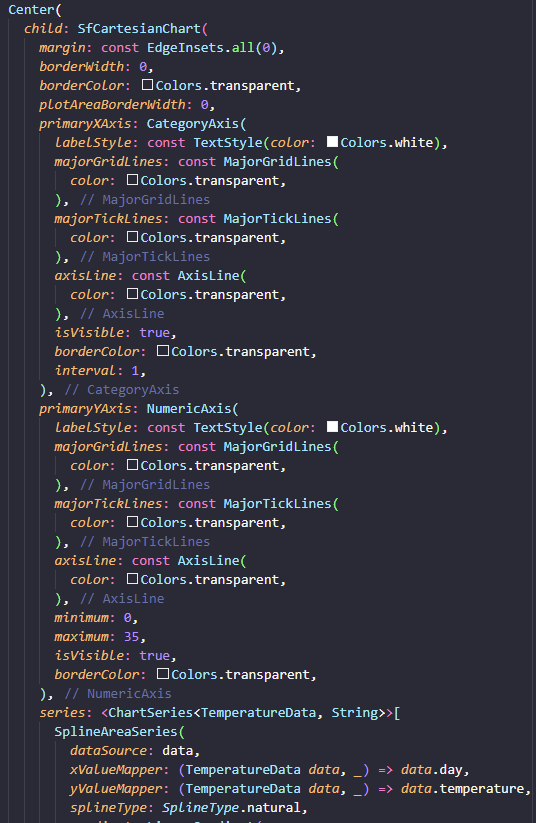
\includegraphics[width=\textwidth]{./pics/CodeSnippetChartDesign.PNG}
\end{minipage}
\begin{minipage}[c]{0.5\textwidth}
    \label{fig:CodeSnippetGraph}
    Dieses Code-Snippet zeigt einen kleinen Einblick wie man einen Graphen designed und mit seinen dazugehörigen 
    Daten befüllt. Ein Graph braucht eine bestimtme Art von Liste durch die er befüllt wird. Die Daten 
    die sich in dieser Liste befinden werde vorher von der Logik durch die HTTP-Request abgefragt und für jeden Graphen einzeln
    aufbereitet um die Daten anschaulich darzustellen.
\end{minipage}
\end{figure}
\newline 
Da der die Sinus-Grpahen jedem Tag nur einen druchschnitts Wert zuordnen um somit die Darstellung übersichtlicher
zu gestalten wird davor für jeden Tag ein Durschnittswert berechnet. Da das Backend um Bits zu sparen nur einen Epoch-Timestamp übergibt
muss dies auch vorher aufbereitet werden.


\newpage
\subsection*{Umsetzung Backend:}
\subsubsection*{Generelle Funktionsweise:}
Die generelle Funktionsweise des Backends basiert auf zwei TTGO-ESP32-LoRa  \newline Mikroprozessoren. 
Einer dieser Mikrochips(Sender) hat 4 verbaute Sensoren darunter:

\begin{itemize}
  \item Temperatursensor
  \item Ph-Sensor
  \item NTU-Trübungssensor
  \item Beschleunigungssensor  
\end{itemize}

Die Sensoren wurden über die vom ESP32 zur Verfügung gestellten Pins angelötet. 
Der Trübungssensor wurde bei einem ADC-Pin (Analog-Digital-Converter) angelötet, 
ebenso wie der Ph-Sensor, der Temperatursensor ist bei einem GPIO (General Purpose Input/Output) angebracht und der Beschleunigungssensor bei einem SDA(serial data) und dem SCL(serial clock) Anschluss. 
Der ESP32(Sender) wird alle 3 Stunden aus seinem Sleep-Zustand aufgeweckt und nimmt eine Messung der Daten vor. Er befindet sich während er inaktiv ist im Sleep damit er noch Stromsparender agiert da er nicht an einer Steckdose angebracht ist sondern mit einer externen Batterie betrieben wird.
Diese Daten werden direkt nach der Messung an den anderen ESP32(Reciever) gesendet. 
Die Daten werden nicht auf dem im Wasser schwimmenden Sender gespeichert da dieser äußerst stromsparend vorgehen soll. 
Die Messwerte werden mittels LoRa-Funk-System welches lokal an dem ESP32 verbaut ist an den Reciever gesendet und dort bei Erhalt mit einem Epoch-Timestamp versehen und in das SPIFF-File-System gespeichert. 
Das äußerst kleine Speichersystem ermöglicht eine Speicherung der Daten in einem Intervall von allen 3 Stunden über 1 Jahr durchgehend. 
Die Daten werden mittels Web-Sockets(für die Live-Daten-Aktualisierung) bereitgestellt und mit einem http-Request der alle Daten an das Frontend übergibt falls das Fenster mit den Zeit-Diagrammen aufgerufen wird um sie in die jeweiligen Diagramme einzufügen. 
Die dazu benötigten Libraries um dies alles in C umzusetzen sind unter „Technologien| Software“ zu finden. 

\newpage
Die Daten die für eine Routine-Übertragung alle 3 Stunden nötig sind, lauten:

\begin{itemize}
  \item Datum
  \item Temperatur
  \item Ph-Wert
  \item NTU-Wert
\end{itemize}

Die Daten des Beschleunigungssensors werden nicht übertragen, um Speicherplatz zu sparen, die Aktualisierungsgeschwindigkeit 
zu erhöhen und eine Echt-Zeit-Benachrichtigung zu ermöglichen, sondern der Sender sendet eine extra Benachrichtigung falls 
der Beschleunigungssensor Werte erreicht hat die auf verdächtige Aktivitäten im Wasser hinweisen. 
Der (Reciever) ESP32 ist  mit dem W-Lan verbunden und permanent eingeschaltet um die Daten 24 Stunden 7 Tage 
in der Woche zu erhalten zu verarbeiten und für das Frontend für eine http-Request bereitzustellen. 


\subsubsection*{Funktion von LoRa in diesem Projekt:}

Die Kommunikationstechnologie, die auf der Basis von Spread-Spectrum-Techniken entwickelt wurde ermöglicht eine drahtlose 
Kommunikation über große Entfernungen bei niedriger Leistungsaufnahme. 
In deinem Fall werden die Daten von drei Sensoren (Temperatursensor, pH-Sensor und NTU-Trübungssensor) mithilfe eines \newline ESP32-Mikrocontrollers und eines LoRa-Transceivers an einen zweiten ESP32, der als Empfänger fungiert, übertragen.


Hier ist das Grundkonzept, wie LoRa funktioniert und die Daten überträgt:

\begin{itemize}
  \item Sensoren erfassen Daten: Die drei Sensoren (Temperatur, pH und NTU-Trübung) erfassen Umgebungsdaten und übermitteln diese an den ESP32-Mikrocontroller.
  \item Datenverarbeitung: Der ESP32-Mikrocontroller verarbeitet die empfangenen Daten, konvertiert sie in ein geeignetes Format und erstellt ein Datenpaket. Dieses Paket enthält die Sensordaten.
  \item LoRa-Modulation: Der LoRa-Transceiver, der am ESP32 angeschlossen ist, wandelt das Datenpaket in ein Funksignal um, das für die Übertragung über das LoRa-Protokoll geeignet ist. LoRa verwendet eine Chirp Spread Spectrum (CSS)-Technologie, bei der die Frequenz des Funksignals kontinuierlich über eine bestimmte Bandbreite variiert. Diese Technik erhöht die Störfestigkeit und ermöglicht eine effiziente Nutzung des Funkspektrums.
  \item Datenübertragung: Das modulierte Funksignal wird über die LoRa-Antenne ausgesendet und kann über große Entfernungen übertragen werden. LoRa ist besonders für Anwendungen mit geringem Energieverbrauch und geringer Datenrate geeignet.
  \item Empfang des Funksignals: Der zweite ESP32, der als Empfänger fungiert, ist ebenfalls mit einem LoRa-Transceiver und einer Antenne ausgestattet. Dieser empfängt das Funksignal, das von der Senderantenne ausgesendet wurde.
  \item Demodulation und Datenextraktion: Der LoRa-Transceiver am Empfänger demoduliert das empfangene Funksignal und extrahiert das ursprüngliche Datenpaket. Dabei wird die Spread-Spectrum-Technik rückgängig gemacht, um die übertragenen Informationen zurückzugewinnen.
  \item Datenverarbeitung: Der empfangende ESP32-Mikrocontroller verarbeitet das extrahierte Datenpaket, um die Daten der einzelnen Sensoren (Temperatur, pH und NTU-Trübung) zu erhalten. Anschließend werden die Daten dann für die Zugriffe des Frontends vorbereitet.
\end{itemize}
